%Use one of the two documentclass lines depending on aspect ratio needed
% for 4x3 aspect ratio slides
%\documentclass{beamer}
%for 16x9 (modern wide screen) aspect ratio slides
\documentclass[aspectratio=169]{beamer}
\usepackage{breqn}
\usepackage{mathtools}
\usepackage[authordate,bibencoding=auto,strict,backend=biber,natbib]{biblatex-chicago}
\addbibresource{references.bib}
\usepackage{bm}

\usepackage{tikz}
\usepackage{tikz-3dplot}
\usetikzlibrary{positioning, fit, shapes, arrows.meta}
\usepackage{subfigure}
\usepackage{tikzit}
\usepackage{etoolbox} % for \ifnumcomp
\usepackage{listofitems} % for \readlist to create arrays

\tikzset{>=latex} % for LaTeX arrow head
\colorlet{myred}{red!80!black}
\colorlet{myblue}{blue!80!black}
\colorlet{mygreen}{green!60!black}
\colorlet{mydarkred}{myred!40!black}
\colorlet{mydarkblue}{myblue!40!black}
\colorlet{mydarkgreen}{mygreen!40!black}
\tikzstyle{node}=[very thick,circle,draw=myblue,minimum size=22,inner sep=0.5,outer sep=0.6]
\tikzstyle{connect}=[->,thick,mydarkblue,shorten >=1]
\tikzset{ % node styles, numbered for easy mapping with \nstyle
  node 1/.style={node,mydarkgreen,draw=mygreen,fill=mygreen!25},
  node 2/.style={node,mydarkblue,draw=myblue,fill=myblue!20},
  node 3/.style={node,mydarkred,draw=myred,fill=myred!20},
}
\def\nstyle{int(\lay<\Nnodlen?min(2,\lay):3)} % map layer number onto 1, 2, or 3

\newcommand{\ket}[1]{\left|#1\right\rangle}

\tdplotsetmaincoords{60}{-20}
\renewcommand{\P}{\mathcal{P}}
\renewcommand{\emph}[1]{\textbf{\textit{#1}}}
% Oxford Maths theming
\usetheme{oxfordmaths}

% \newtheorem{theorem}{Theorema}
% \newtheorem{lemma}[theorem]{Lemma}
% \newtheorem{corollary}[theorem]{Corollarium}
\newtheorem{prop}{Proposition}

% Set author etc info
\title[Tensor ZXW] %short version of title for slide footer
{Tensor Network Contraction Using ZXW Calculus} %full title for titlepage
\author{Yuhao Han}
\institute{Mathematical Institute\\University of Oxford}
\date[\today]  %short date for slide footer
{} %main date for title page,
                        %can overload it to show say 'Conference X, Date Y'


%% Now for the actual slides %%
\begin{document}

\begin{frame}[plain]
  \titlepage
\end{frame}


\begin{frame}
	\frametitle{Tensor Network}

	Tensor Network is a graph representation of high-dimensional matrices (or so called tensors). \cite{penrose1971applications}
	In this slide the tensor network are reading from top to bottom.
	
	In particular, the vertices denote tensors, and the edges denote the indices of the tensors.

	$$
	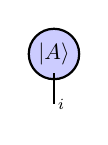
\begin{tikzpicture}[baseline=-0.1ex, scale=0.8, every node/.style={transform shape}]
      % Central tensor node
		\draw[fill=blue!20, thick] (0,0.4) circle (0.4) node (A) {$\ket{A}$};
      % Physical index (pointing up)
      \draw[thick] (A.south) -- (0,-0.4) node[right=-2pt] {\scriptsize $i$};
      % Virtual indices (left and right bonds)
    \end{tikzpicture} =
	\begin{pmatrix}
		1 \\ 
		0
	\end{pmatrix}, \qquad 
	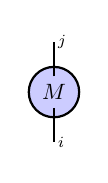
\begin{tikzpicture}[baseline=-0.1ex, scale=0.8, every node/.style={transform shape}]
      % Central tensor node
		\draw[fill=blue!20, thick] (0,0.) circle (0.4) node (A) {$M$};
      % Physical index (pointing up)
      \draw[thick] (A.south) -- (0,-0.8) node[right=-2pt] {\scriptsize $i$};
      \draw[thick] (A.north) -- (0,0.8) node[right=-2pt] {\scriptsize $j$};
      % Virtual indices (left and right bonds)
    \end{tikzpicture} =
	\begin{pmatrix}
		1  & 2\\ 
		2  & 3
	\end{pmatrix}
	$$
	
	The edges are just indices of tensor, as
	$$
	A_0 = 1, A_1 = 0, M^0_0 = 1, M^0_1 = 2, M^1_0 = 2, M^1_1 = 3.
	$$
\end{frame}

\begin{frame}
	\frametitle{Tensor Network}

	The edges connecting the vertices denotes summing over the indices

	$$
	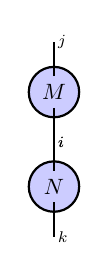
\begin{tikzpicture}[baseline=-0.1ex, scale=0.8, every node/.style={transform shape}]
      % Central tensor node
	\draw[fill=blue!20, thick] (0,1.5) circle (0.4) node (A) {$M$};
      % Physical index (pointing up)
      \draw[thick] (A.south) -- (0,0.7) node[right=-2pt] {\scriptsize $i$};
      \draw[thick] (A.north) -- (0,2.3) node[right=-2pt] {\scriptsize $j$};
      % Virtual indices (left and right bonds)
	\draw[fill=blue!20, thick] (0,0) circle (0.4) node (A) {$N$};
      % Physical index (pointing up)
      \draw[thick] (A.north) -- (0,0.7) node[right=-2pt] {\scriptsize $i$};
      \draw[thick] (A.south) -- (0,-0.8) node[right=-2pt] {\scriptsize $k$};
    \end{tikzpicture} \qquad = \qquad
	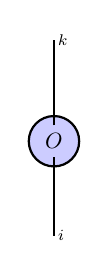
\begin{tikzpicture}[baseline=-0.1ex, scale=0.8, every node/.style={transform shape}]
      % Central tensor node
	\draw[fill=blue!20, thick] (0,0.7) circle (0.4) node (A) {$O$};
      % Physical index (pointing up)
      \draw[thick] (A.south) -- (0,-0.8) node[right=-2pt] {\scriptsize $i$};
      \draw[thick] (A.north) -- (0,2.3) node[right=-2pt] {\scriptsize $k$};
      % Virtual indices (left and right bonds)
    \end{tikzpicture}
	$$
	And $O^k_j = \sum_i M^j_i N^i_j$: This is exactly the matrix multiplication of $M$ and $N$.
\end{frame}

\begin{frame}
	\frametitle{Tensor Network}

	The nodes putting next to each other denotes tensor product.

	$$
	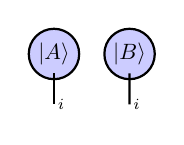
\begin{tikzpicture}[baseline=-0.1ex, scale=0.8, every node/.style={transform shape}]
      % Central tensor node
		\draw[fill=blue!20, thick] (0,0.4) circle (0.4) node (A) {$\ket{A}$};
      % Physical index (pointing up)
      \draw[thick] (A.south) -- (0,-0.4) node[right=-2pt] {\scriptsize $i$};
      % Virtual indices (left and right bonds)
	\draw[fill=blue!20, thick] (1.2,0.4) circle (0.4) node (B) {$\ket{B}$};
      % Physical index (pointing up)
      \draw[thick] (B.south) -- (1.2,-0.4) node[right=-2pt] {\scriptsize $i$};
	  \end{tikzpicture} = \ket{A} \otimes \ket{B} 
	$$
	Precisely, if 
	If $\ket{A} \in V $, and for demonstration purpose $\ket{A}= \begin{pmatrix}
		a \\ 
		b
		\end{pmatrix}$, $\ket{B} \in W $ and $\ket{B}= \begin{pmatrix}
		c \\ 
		d
	\end{pmatrix}$. 
	 We can pick an alphabetical order for the basis $V \otimes W$ and $\ket{A} \otimes \ket{B} = \begin{pmatrix}
		ac \\
		ad \\
		bc \\
		bd
	\end{pmatrix}$.
\end{frame}

\begin{frame}
	\frametitle{Tensor Network}
	
	Basically almost all operations \cite{coecke2016categoricalquantummechanicsi} on finite-dimentional vector space can be represented by some ``rules'' of tensor network.
	For example
	transpose can be represented as 
	\begin{figure}[htbp]
		\centering
		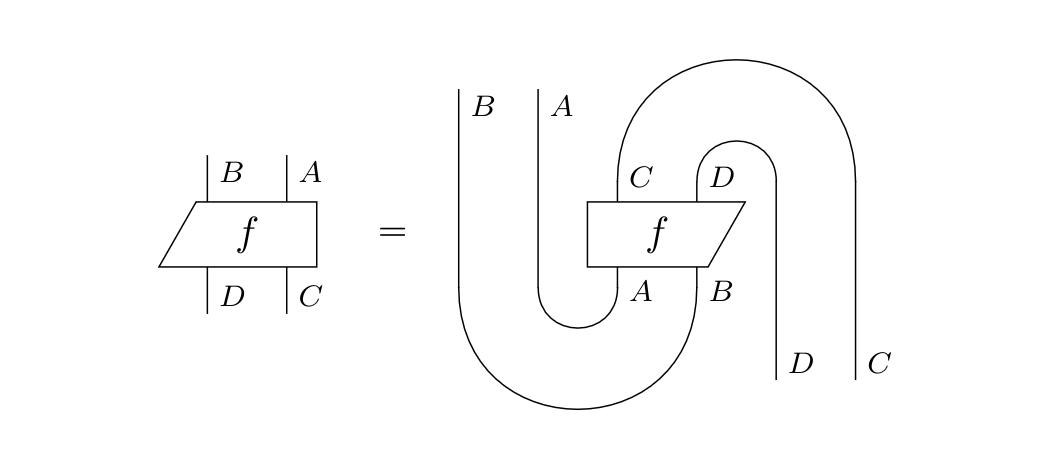
\includegraphics[width=0.6\textwidth]{./transpose.png}
	\end{figure}

	In this sense, tensor network is equivalent to our usual notation of linear algebra.
	If representing the category of finite dimensional vector space as $\textbf{FHilb}$, the tensor network is its string diagram.
\end{frame}

\begin{frame}[allowframebreaks]
	\frametitle{Application of Tensor Network}
	Tensor network is a very powerful tool.

	\begin{figure}[htbp]
		\centering
		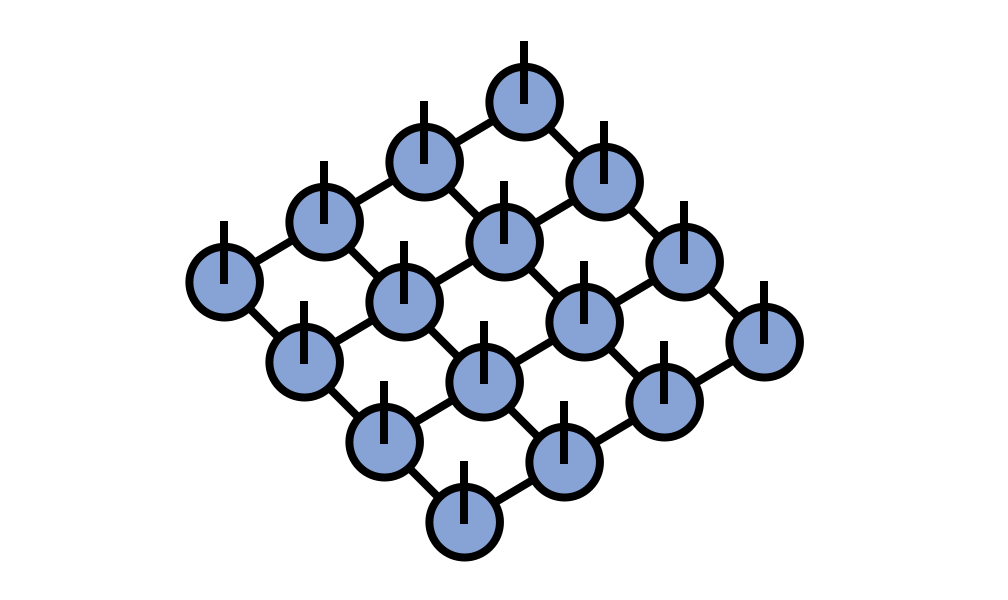
\includegraphics[width=0.4\textwidth]{./PEPS.png}
		\caption{Projected entangled paried State (PEPS) \cite{Patra_2025}, representing an ansatz for quantum wavefunctions}
		\label{fig:Peps State}
	\end{figure}
	\begin{figure}[htbp]
		\centering
		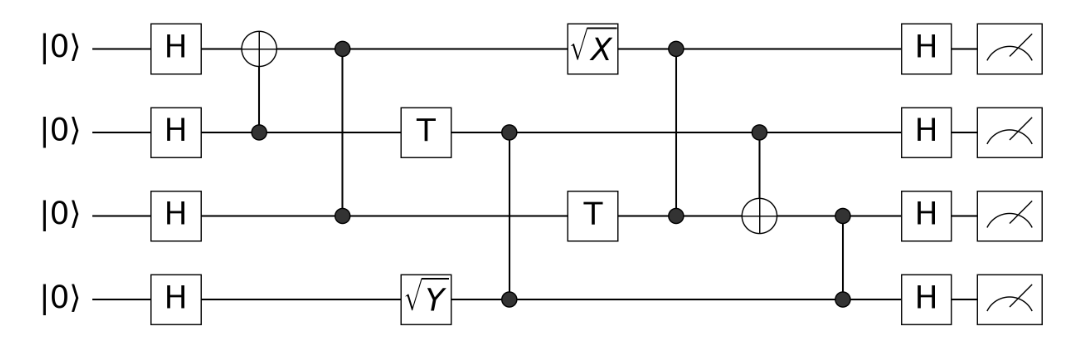
\includegraphics[width=0.6\textwidth]{./quantum-circuit.png}
		\caption{A quantum circuit as a tensor network}
	\end{figure}
	They can be very complicated too. \cite{Gray_2021}
	\begin{figure}[htbp]
		\centering
		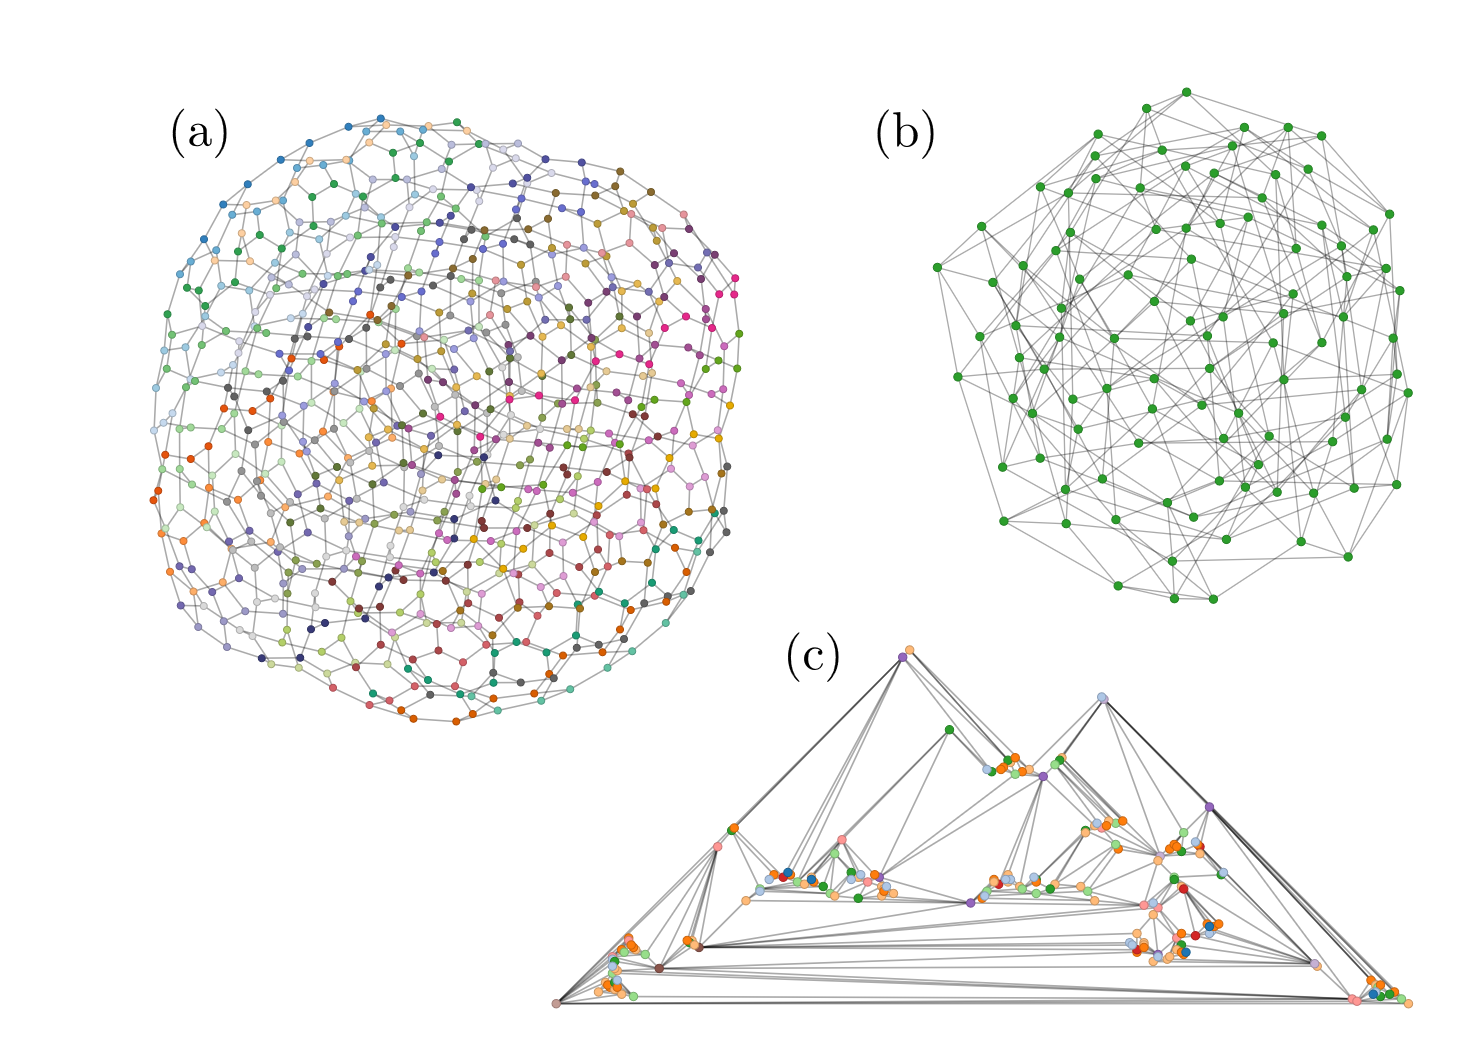
\includegraphics[width=0.5\textwidth]{./complicated-tensor.png}
		\caption{Tensor network for (a) random qunatum circuit, (b) SAT probelm, (c) the statistical-mechanical evaluation of knot invariants}
	\end{figure}
\end{frame}

\begin{frame}
	\frametitle{Tensor Contraction}
	Tensor contraction is basically the process of evaluating a tensor network.
	Assuming all our edges are of dimension $D$.
	$$
	O = 
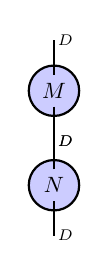
\begin{tikzpicture}[baseline=-0.1ex, scale=0.8, every node/.style={transform shape}]
      % Central tensor node
	\draw[fill=blue!20, thick] (0,1.5) circle (0.4) node (A) {$M$};
      % Physical index (pointing up)
      \draw[thick] (A.south) -- (0,0.7) node[right=-2pt] {\scriptsize $D$};
      \draw[thick] (A.north) -- (0,2.3) node[right=-2pt] {\scriptsize $D$};
      % Virtual indices (left and right bonds)
	\draw[fill=blue!20, thick] (0,0) circle (0.4) node (A) {$N$};
      % Physical index (pointing up)
      \draw[thick] (A.north) -- (0,0.7) node[right=-2pt] {\scriptsize $D$};
      \draw[thick] (A.south) -- (0,-0.8) node[right=-2pt] {\scriptsize $D$};
  \end{tikzpicture}, \qquad \text{and} \qquad
O^k_j = \sum_i M^j_i N^i_j
	$$
	Computing one entry of $O^k_j$ takes $O(D)$ time, and computing the whole matrix $O$ takes $O(D^3)$ time (and $O(D^2)$ times) to store it.

\end{frame}

\begin{frame}[allowframebreaks]
	\frametitle{Tensor Contraction}
	For contracting an arbitrary tensor network, the order matters.
	The time complexity of the contraction is $O(\exp{n+1})$, where $n$ is the maximum number of order in the intermediate vertices. (Order is number of edged connecting to it.) \cite{waintal2026competequantumcomputerslecture}

	\begin{figure}[htbp]
		\centering
		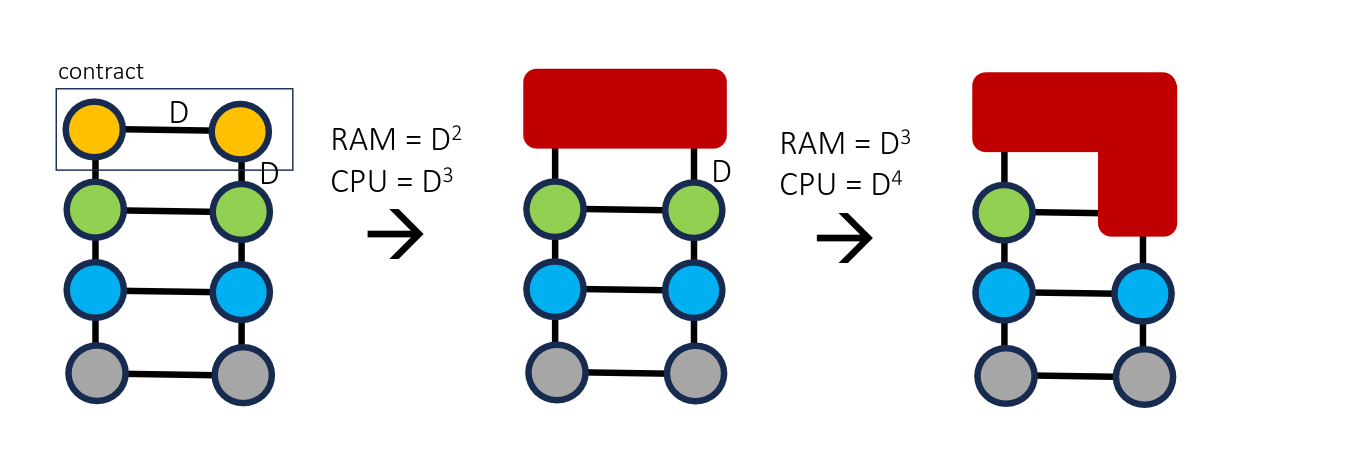
\includegraphics[width=0.8\textwidth]{./contraction1.png}
	\end{figure}

	\begin{figure}[htbp]
		\centering
		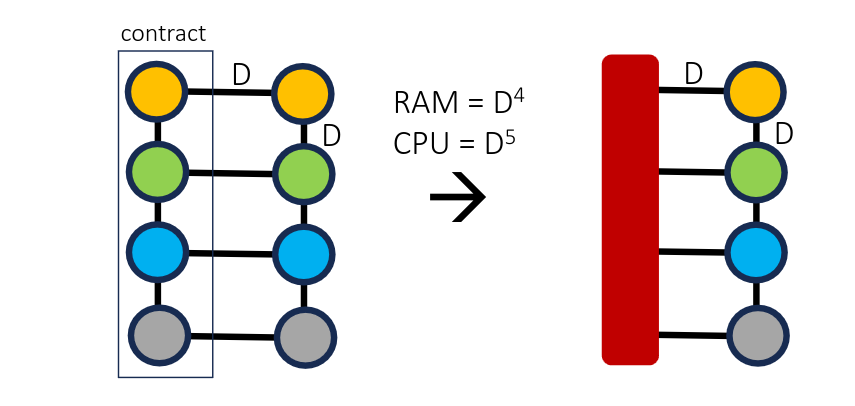
\includegraphics[width=0.5\textwidth]{./contraction2.png}
	\end{figure}

	In general, finding the optimal order for tensor contraction is NP-hard, and the best we can do is to find some good heuristics.
\end{frame}

\begin{frame}[allowframebreaks]
	\frametitle{ZXW calculus}
	ZXW calculus is a particular flavour of tensor network, that uses some tensors as generators and a set of rewrite rules \cite{wang2026completenessqufinitezxwcalculus}

	\begin{figure}[htbp]
		\centering
		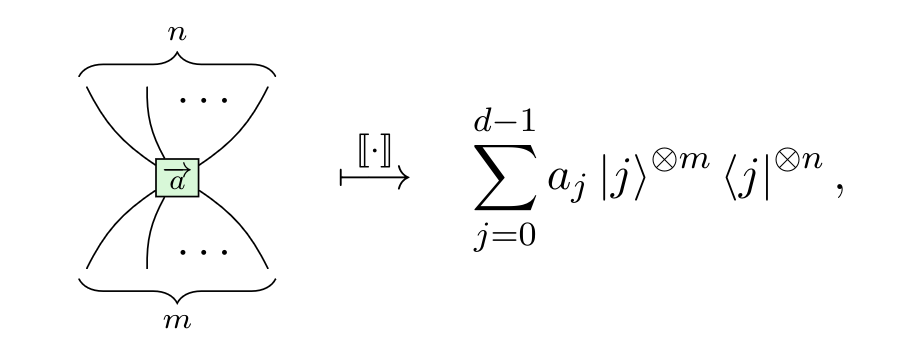
\includegraphics[width=0.5\textwidth]{zbox.png}
		\caption{Z box}
		\label{fig:Z box}
	\end{figure}
	\begin{figure}[htbp]
		\centering
		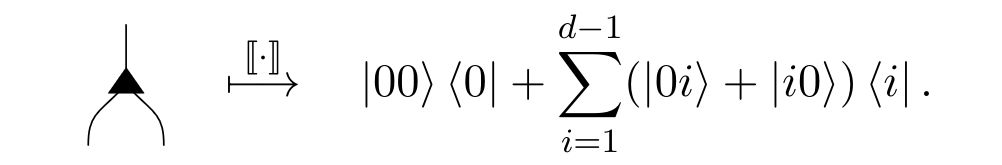
\includegraphics[width=0.5\textwidth]{WNode.png}
		\caption{W node}
	\end{figure}
	\begin{figure}[htbp]
		\centering
		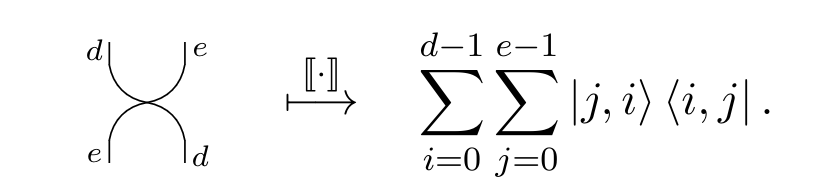
\includegraphics[width=0.5\textwidth]{swap.png}
		\caption{Swap}
	\end{figure}
	\begin{figure}[htbp]
		\centering
		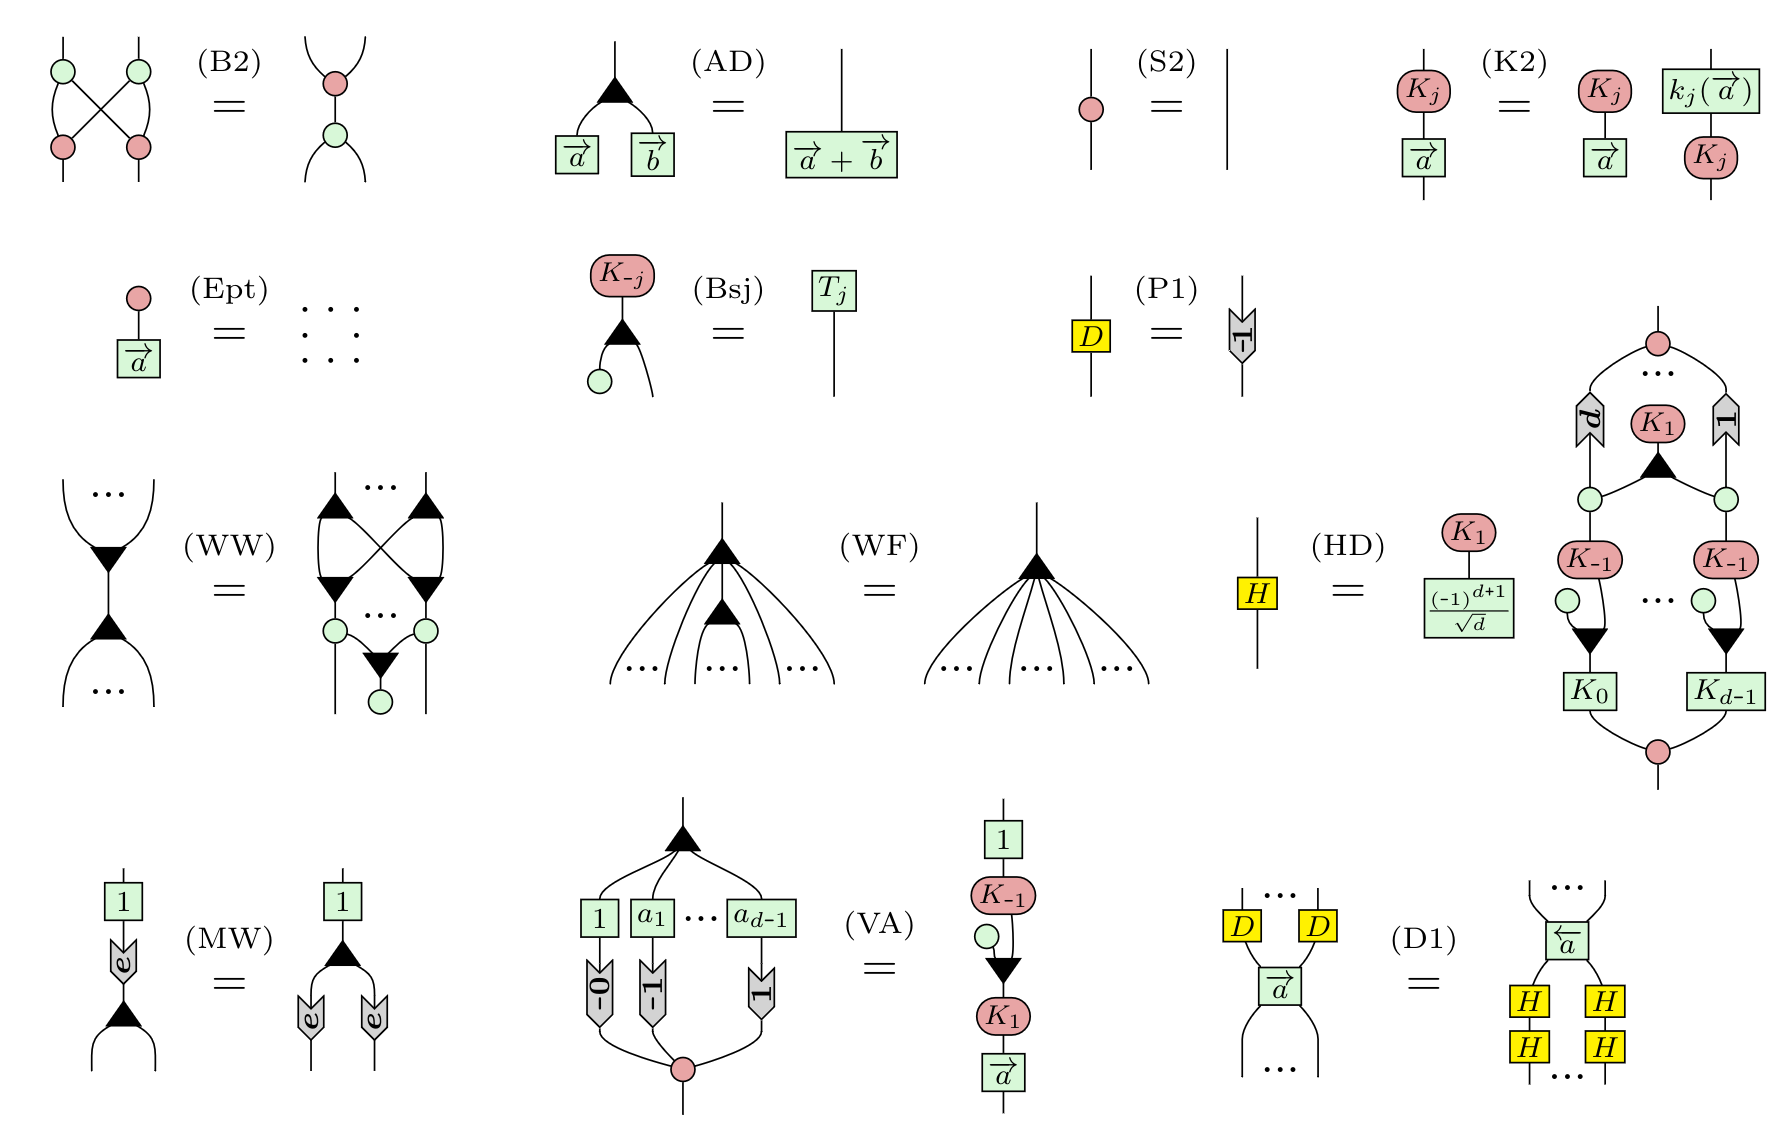
\includegraphics[width=0.5\textwidth]{rewrite.png}
		\caption{A list of rewriting rules}
	\end{figure}

	Importantly, ZXW-calculus is universal and complete,
	\begin{enumerate}
		\item any tensor or linear transformation can be represented by a ZXW-diagram, 
		\item and any equation involving linear maps that can be derived using linear algebra can also be derived using ZXW-diagrams and the rewrite rules.
	\end{enumerate}
	In the jargon of category theory, the functor $F: \mathbf{FHilt} \rightarrow \mathbf{ZXW}$, which we called the interpretation functor, is full and faithful. \cite{wang2026completenessqufinitezxwcalculus}
\end{frame}

\begin{frame}[allowframebreaks]
	\frametitle{Usefulness of ZXW in Contracting Tensor Network}
	Notable example is quantum teleportation.

	\begin{figure}[htbp]
		\centering
		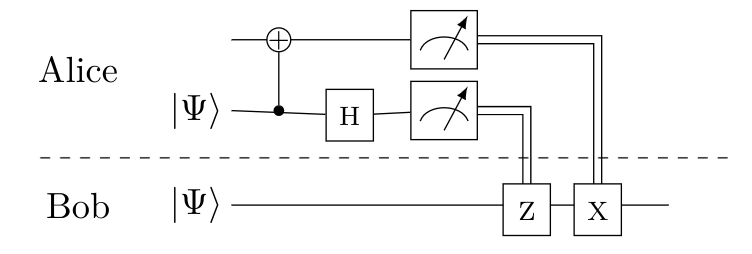
\includegraphics[width=0.6\textwidth]{teleportation_circuit.png}
	\end{figure}
	\begin{figure}[htbp]
		\centering
		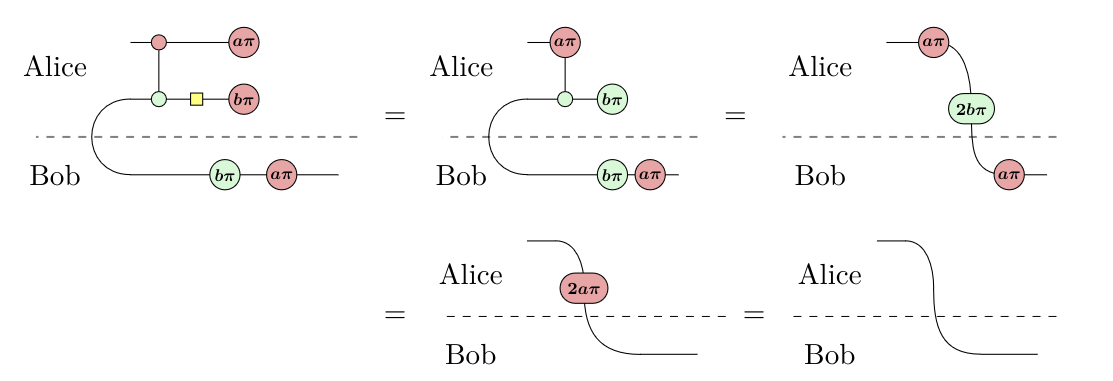
\includegraphics[width=0.6\textwidth]{teleportation-zx.png}
	\end{figure}
\end{frame}

\begin{frame}[allowframebreaks]
	\frametitle{Local Complementation}
	Local complementation \cite{KissingerWetering2024Book} of a graph $G$ on a vertex $v$, which we write as $G\star v$, is a new graph has the same vertices as $G$ but with the edges between the neighbors of $v$ flipped.
	\begin{figure}[htbp]
		\centering
		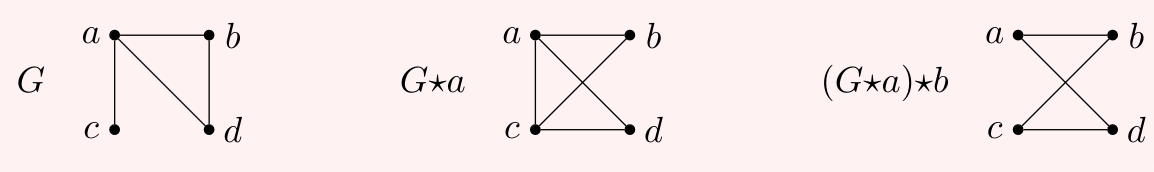
\includegraphics[width=0.6\textwidth]{local_complementation.png}	
	\end{figure}

	For a specific type of tensor network, called graph state, we can use local complementation to rewrite the tensor network.
	\begin{figure}[htbp]
		\centering	
		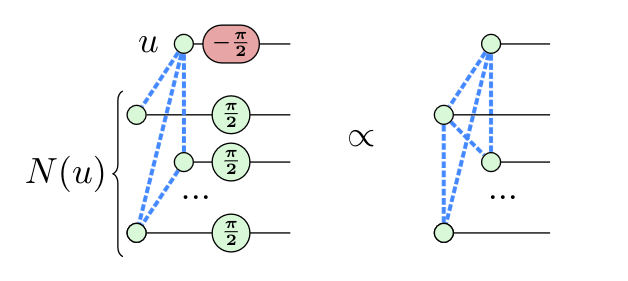
\includegraphics[width=0.6\textwidth]{local-complementation-zx.png}
	\end{figure}

	The number of edges are reduced: so hopefully contraction can be easier.

	Specifically, we can use local complementation to reduce the tree-width of the graph, which is a measure of how hard it is to contract the tensor network.
\end{frame}

\begin{frame}
	\frametitle{Current Work}	
	\begin{enumerate}
		\item The previous graph state is a very special type of tensor network, where each edge is of dimension 2. We can try to expand it to more general tensor network using q-finite ZXW calculus.
		\item Similar to local complementation is pivoting, which may also drastically reduce the tree-width of the graph. 
	\end{enumerate}
\end{frame}

\begin{frame}[allowframebreaks]
        \frametitle{References}
        \printbibliography
\end{frame}

\end{document}
